%
% hypergeometrisch.tex
%
% (c) 2021 Prof Dr Andreas Müller, OST Ostschweizer Fachhochschule
%
\section{Hypergeometrische Funktionen
\label{buch:rekursion:section:hypergeometrische-funktion}}
\rhead{Hypergeometrische Funktionen}
Kann man eine Formel für die Lösung $S_n$ der lineare Differenzengleichung
\[
n^3S_{n}
=
16(n-{\textstyle\frac12})(2n^2-2n+1)S_{n-1}
-256(n-1)^3S_3
\]
mit Anfangswerten $S_0=1$ und $S_1=8$ angeben?
Dies scheint auf den ersten Blick unmöglich kompliziert, man kann aber
zeigen, dass
\begin{equation}
S_n
=
\sum_{k=0}^n 
\binom{2n-2k}{n-k}^2 \binom{2k}{k}^2
\label{buch:rekursion:hypergeometrisch:eqn:Sn}
\end{equation}
gilt (\cite[p.~xi]{buch:ab}).
Die Lösung ist also eine Summe von Summanden, die sehr viel einfacher
aussehen und vor allem die besondere Eigenschaft haben, dass die
Quotienten aufeinanderfolgender Terme rationale Funktionen von $k$
sind.

\begin{definition}
Ein Folge heisst {\em hypergeometrisch}, wenn der Quotient aufeinanderfolgender
\index{hypergeometrische Folge}%
\index{Folge, hypergeometrisch}%
Terme eine rationale Funktion des Folgenindex ist.
\end{definition}

Die Terme der Reihenentwicklungen aller bisher behandelten speziellen
Funktionen waren hypergeometrisch.
Im aktuellen Abschnitt soll daher die Klasse der sogenannten
hypergeometrischen Funktionen untersucht werden, die durch diese
Eigenschaft charakterisiert sind.

In Abschnitt~\ref{buch:rekursion:hypergeometrisch:binomialkoeffizienten}
wird klar, dass Folgen, deren Terme aus Fakultäten und Binomialkoeffizienten
immer hypergeometrisch sind.
\index{Binomialkoeffizient}%
Die Untersuchung der geometrischen Reihe in
Abschnitt~\ref{buch:rekursion:hypergeometrisch:geometrisch}
\index{geometrische Reihe}%
\index{Reihe, geometrische}%
motiviert die Namensgebung.
Abschnitt~\ref{buch:rekursion:hypergeometrisch:reihen}
definiert den Begriff der hypergeometrischen Reihe und zeigt, 
wie sie in eine Standardform gebracht werden können.
In Abschnitt~\ref{buch:rekursion:hypergeometrisch:beispiele}
schliesslich wird an Hand von Beispielen gezeigt, wie bekannte
Funktionen als hypergeometrische Funktionen interpretiert werden können.

%
% Quotienten von Binomialkoeffizienten
%
\subsection{Quotienten von Binomialkoeffizienten
\label{buch:rekursion:hypergeometrisch:binomialkoeffizienten}}
Aufeinanderfolgende Terme der Summe
\eqref{buch:rekursion:hypergeometrisch:eqn:Sn}
sollen als Quotienten eine rationale Funktion haben.
Dies ist eine allgemeine Eigenschaft von Folgen, die durch Fakultäten
oder Binomialkoeffizienten definiert sind, wie die beiden folgenden
Sätze zeigen.

\begin{satz}
\index{Satz!Quotienten von Fakultäten}%
\label{buch:rekursion:hypergeometrisch:satz:fakquo}
Der Quotient aufeinanderfolgender Folgenglieder
der Folge $c_k=(a+bk)!$ ist der ein Polynom vom Grad $b$.
\end{satz}
\begin{proof}[Beweis]
\begin{align*}
\frac{c_{k+1}}{c_k}
&=
\frac{(a+b(k+1))!}{(a+bk)!}
=
\frac{(a+bk+b)!}{(a+b)!}
\\
&=
(a+bk+1)(a+bk+2)\cdots(a+bk+b)
=
(a+bk+1)_b.
\end{align*}
Das Pochhammer-Symbol hat $b$ Faktoren, es ist ein Polynom vom Grad $b$.
\end{proof}
\index{Pochhammer-Symbol}%

\begin{satz}
\index{Satz!Quotienten von Binomialkoeffizienten}%
\label{buch:rekursion:hypergeometrisch:satz:binomquo}
Die Quotienten aufeinanderfolgender Werte der Binomialkoeffizienten
\[
f_k
=
\binom{a+bk}{c+dk}
\]
ist eine rationale Funktion von $k$ mit Zähler- und Nennergrad $b$.
\end{satz}

\begin{proof}[Beweis]
Indem man die Binomialkoeffizienten mit Fakultäten als
\[
\binom{a+bk}{c+dk}
=
\frac{(a+bk)!}{(c+dk)!(a-c+(b-d)k)!}
\]
ausschreibt, findet man mit
Satz~\ref{buch:rekursion:hypergeometrisch:satz:fakquo}
für die Quotienten
\begin{align}
\frac{f_{k+1}}{f_k}
&=
\frac{(a+bk+1)_b}{(c+dk+1)_d\cdot(a-c+(b-d)k+1)_{b-d}}.
\label{buch:rekursion:eqn:binomquotient}
\end{align}
Die Pochhammer-Symbole sind Polynome vom Grad $b$, $d$ bzw.~$b-d$.
Insbesondere ist auch das Nenner-Polynom vom Grad $d+(b-d)=b$.
\end{proof}

Aus den Sätzen~\ref{buch:rekursion:hypergeometrisch:satz:fakquo}
und
\ref{buch:rekursion:hypergeometrisch:satz:binomquo}
folgt jetzt sofort, dass auch der Quotient aufeinanderfolgender
Summanden der Summe~\eqref{buch:rekursion:hypergeometrisch:eqn:Sn}
eine rationale Funktion von $k$ ist.

%
% Die geometrische Reihe
%
\subsection{Die geometrische Reihe
\label{buch:rekursion:hypergeometrisch:geometrisch}}
Die Reihe
\[
f(q)
=
\sum_{k=0}^\infty aq^k
\]
heisst die {\em geometrische Reihe} ist besonders einfache
Reihe mit einer hypergeometrischen Folge von Termen.
\index{geometrische Reihe}%
\index{Reihe!geometrische}%
Die Partialsummen 
\[
S_n
=
\sum_{k=0}^n aq^k
\]
können aus der Differenz
\begin{equation}
(1-q)S_n
=
S_n - qS_n
=
\sum_{k=0}^n aq^k
-
\sum_{k=1}^{n+1} aq^k
=
a -aq^{n+1}
\label{buch:rekursion:hypergeometrisch:eqn:qsumme}
\end{equation}
berechnet werden, die man nach
\begin{equation}
S_n 
=
a\frac{1-q^{n+1}}{1-q}
\label{buch:rekursion:hypergeometrisch:eqn:geomsumme}
\end{equation}
auflösen kann.
Für $q<1$ geht $q^n\to 0$ und damit konvergiert
$S_n$  gegen
\[
\sum_{k=0}^\infty aq^k
=
a\frac{1}{1-q}.
\]

Die geometrische Reihe ist charakterisiert dadurch, dass aufeinanderfolgende
Terme den gleichen Quotienten
\[
\frac{aq^{k+1}}{aq^k}
=
q
\]
haben.
\index{geometrische Reihe}%
\index{Reihe, geometrische}%
Die Berechnung der Summe in 
\eqref{buch:rekursion:hypergeometrisch:eqn:qsumme}
beruht darauf, dass die Multiplikation mit $q$ einen ``anderen''
Teil der Summe ergibt, der sich in der Differenze weghebt.

%
% Hypergeometrische Reihen
%
\subsection{Hypergeometrische Reihen
\label{buch:rekursion:hypergeometrisch:reihen}}
Es ist plausibel, dass eine etwas lockerere Bedingung an die
Quotienten aufeinanderfolgender Terme einer Reihe immer noch
ermöglichen wird, interessante Aussagen über die durch die
Reihe beschriebenen Funktionen zu machen.

\begin{definition}
\label{buch:rekursion:hypergeometrisch:def:allg}
Eine durch die Reihe
\[
f(x) = \sum_{k=0}^\infty a_k x^k
\]
definierte Funktion $f(x)$ heisst {\em hypergeometrisch},
wenn der Quotient aufeinanderfolgender
\index{hypergeometrisch}
\index{Reihe!hypergeometrisch}
Koeffizienten eine rationale Funktion von $k$ ist,
wenn also
\[
\frac{a_{k+1}}{a_k}
=
\frac{p(k)}{q(k)}
\]
mit Polynomen $p(k)$ und $q(k)$ ist.
\end{definition}

%
% Beispiele von hypergeometrischen Funktionen
%
\subsubsection{Beispiele von hypergeometrischen Funktionen}
Die geometrische Reihe ist natürlich eine hypergeometrische Reihe,
wobei $p(k)/q(k)=1$ ist.
Etwas interessanter ist die Exponentialfunktion, die durch die Taylor-Reihe
\index{Taylor-Reihe}%
\[
e^x = \sum_{k=0}^\infty \frac{x^k}{k!}
\]
dargestellt werden kann.
Der Quotient aufeinanderfolgender Koeffizienten ist
\[
\frac{a_{k+1}}{a_k}
=
\frac{1/(k+1)!}{1/k!}
=
\frac{k!}{(k+1)!}
=
\frac{1}{k+1},
\]
eine rationale Funktion mit Zählergrad $0$ und Nennergrad $1$.

Die Kosinus-Funktion wird durch die Taylor-Reihe
\[
\cos x = \sum_{k=0}^\infty \frac{(-1)^k}{(2k)!} x^{2k}
\]
dargestellt.
Als Potenzreihe in $x$ kann die Kosinus-Reihe nicht hypergeometrisch sein,
die ungeraden Koeffizienten verschwinden und damit undefinierte
Quotienten haben.
Als Reihe in $z=x^2$ ist aber
\[
\sum_{k=0}^\infty \frac{(-1)^k}{(2k)!} z^k
\qquad\Rightarrow\qquad
a_k = \frac{(-1)^k}{(2k)!}
\]
hypergeometrisch, weil der Quotient aufeinanderfolgender Koeffizienten
\[
\frac{a_{k+1}}{a_k}
=
\frac{(-1)^{k+1}}{(2k+2)!}\cdot \frac{(2k)!}{(-1)^k}
=
-\frac{1}{(2k+2)(2k+1)},
\]
eine rationale Funktion mit Zählergrad $0$ und Nennergrad $2$.
Es gibt also eine hypergeometrische Reihe $f(z)$ derart, dass
$\cos x = f(x^2)$ ist.

%
% Die hypergeometrischen Funktione pFq
%
\subsubsection{Die hypergeometrischen Funktionen $\mathstrut_pF_q$}
Die Definition~\ref{buch:rekursion:hypergeometrisch:def:allg}
einer hypergeometrischen Funktion wie auch die Verschiedenartigkeit
der Beispiele kännen den Eindruck vermitteln, dass die diese Klasse
von Funktionen unübersichtlich gross sein könnte.
Dem ist jedoch nicht so.
In diesem Abschnitt soll gezeigt werden, dass alle hypergeometrischen
Funktionen durch die in
Definition~\ref{buch:rekursion:hypergeometrisch:def} definierten
Funktionen $\mathstrut_pF_q$ ausgedrückt werden.
Die hypergeometrischen Funktionen können also vollständig parametrisiert
werden.

Zu diesem Zweick sie
\[
f(x)
=
\sum_{k=0}^\infty a_kx^k
\]
eine hypergeometrische Funktion und
seien $p(k)$ und $q(k)$ zwei Polynome derart, dass
\[
\frac{a_{k+1}}{a_k} = \frac{p(k)}{q(k)}.
\]
Daraus lässt sich der Koeffizient $a_{k+1}$ als
\begin{equation}
a_{k+1}
=
\frac{p(k)}{q(k)}
\cdot
a_k
=
\frac{p(k)}{q(k)}
\cdot
\frac{p(k-1)}{q(k-1)}
\cdot
a_{k-1}
=\dots=
\frac{p(k)}{q(k)}
\frac{p(k-1)}{q(k-1)}
\cdots
\frac{p(1)}{q(1)}
\frac{p(0)}{q(0)}
a_0
\label{buch:rekursion:hypergeometrisch:ak+1}
\end{equation}
berechnen.
Alle Koeffizienten haben also den Faktor $a_0=f(0)$ gemeinsam.

Die Produkte von Quotienten $p(k)/q(k)$ sollen jetzt weiter
vereinfacht werden.
Sei $n$ der Grad von $p(k)$ und $m$ der Grad von $q(k)$.
Dazu nehmen wir an, dass $a_i$, $i=1,\dots,n$ die Nullstellen von $p(k)$ sind
und $b_j$, $j=1,\dots,m$ die Nullstellen von $q(k)$, dass man also
die Polynome als
\begin{align*}
p(k) &= s(k-a_1)(k-a_2)\cdots(k-a_n)
\\
q(k) &= (k-b_1)(k-b_2)\cdots(k-b_m)
\end{align*}
schreiben kann.
Der Faktor $s$ ist nötig, weil die Polynome $p(k)$ und $q(k)$ nicht
notwendigerweise normiert sind.

Um das Produkt der Quotienten zu vereinfachen, nehmen wir für den Moment
an, dass Zähler und Nenner vom Grad $n=m=1$ ist.
Dann ist nach 
\eqref{buch:rekursion:hypergeometrisch:ak+1}
\[
a_{k}
=
s^{k}
\frac{
(k-1-a_1) \cdots (2-a_1)(1-a_1)(0-a_1)
}{
(k-1-b_1) \cdots (2-b_1)(1-b_1)(0-b_1)
}
=
\frac{(-a_1)_k}{(-b_1)_k} s^k.
\]
Die Koeffizienten können daher als Quotienten von Pochhammer-Symbolen
geschrieben werden.
Für Polynome $p(k)$ und $q(k)$ höheren Grades sind die Koeffizienten
von der Form
\[
a_k
=
\frac{(-a_1)_k(-a_2)_k\cdots (-a_n)_k}{(-b_1)_k(-b_2)_k\cdots(-b_m)_k}
s^ka_0.
\]
Jede hypergeometrische Funktion kann daher in der Form
\[
f(x)
=
a_0
\sum_{k=0}^\infty
\frac{(-a_1)_k(-a_2)_k\cdots (-a_n)_k}{(-b_1)_k(-b_2)_k\cdots(-b_m)_k}
s^k
x^k
\]
geschrieben werden.

\begin{definition}
\label{buch:rekursion:hypergeometrisch:def}
Die hypergeometrische Funktion
$\mathstrut_pF_q$ ist definiert durch die Reihe
\[
\mathstrut_pF_q
\biggl(
\begin{matrix}
a_1,\dots,a_p\\
b_1,\dots,b_q
\end{matrix}
;
x
\biggr)
=
\mathstrut_pF_q(a_1,\dots,a_p;b_1,\dots,b_q;x)
=
\sum_{k=0}^\infty
\frac{(a_1)_k\cdots(a_p)_k}{(b_1)_k\cdots(b_q)_k}\frac{x^k}{k!}.
\]
\end{definition}

Da $(1)_k=k!$ hätte die Definition den Nenner $k!$ in der Reihe
auch durch eines der Pochhammer-Symbole ausdrücken können.
Wird dieser Nenner nicht gebraucht, kann man ihn durch einen 
zusätzlichen Faktor $(1)_k$ im Zähler des Bruchs von Pochhammer-Symbolen
kompensieren, wodurch sich der Grad $p$ des Zählers natürlich um $1$
erhöht.

Die oben analysierte Summe für $f(x)$ kann mit der
Definition~\ref{buch:rekursion:hypergeometrisch:def} als
\[
f(x)
=
a_0
\cdot
\mathstrut_{n+1}F_m \biggl(
\begin{matrix}
-a_1,-a_2,\dots,-a_n,1\\
-b_1,-b_2,\dots,-a_m
\end{matrix}; sx
\biggr)
\]
beschrieben werden.

%
% Elementare Rechenregeln
%
\subsubsection{Elementare Rechenregeln}
Die Funktionen $\mathstrut_pF_q$ sind nicht alle unabhängig.
In Abschnitt~\ref{buch:rekursion:hypergeometrisch:stammableitung}
wird gezeigt werden, dass Ableitung und Stammfunktion einer hypergeometrischen
Funktion durch Manipulation der Parameter $a_k$ und $b_k$ bestimmt werden
können.
Viel einfacher sind jedoch die folgenden, aus
Definition~\ref{buch:rekursion:hypergeometrisch:def}
offensichtlichen Regeln:

\begin{satz}[Permutationsregel]
\index{Permutationsregel}%
\index{Satz!Permutationsregel für hypergeometrische Funktionen}%
\label{buch:rekursion:hypergeometrisch:satz:permuationsregel}
Sei $\pi$ eine beliebige Permutation der Zahlen $1,\dots,p$ und $\sigma$ eine
beliebige Permutation der Zahlen $1,\dots,q$, dann ist 
\begin{equation}
\mathstrut_pF_q\biggl(
\begin{matrix}
a_1,\dots,a_p\\b_1,\dots,a_q
\end{matrix}
;x
\biggr)
=
\mathstrut_pF_q\biggl(
\begin{matrix}
a_{\pi(1)},\dots,a_{\pi(p)}\\b_{\sigma(1)},\dots,b_{\sigma(q)}
\end{matrix}
;x
\biggr).
\label{buch:rekursion:hypergeometrisch:eqn:permuationsregel}
\end{equation}
\end{satz}

\begin{satz}[Kürzungsformel]
\index{Kürzungsregel}%
\index{Satz!Kürzungsformel für hypergeometrische Funktionen}%
\label{buch:rekursion:hypergeometrisch:satz:kuerzungsregel}
Stimmt einer der Koeffizienten $a_k$ mit einem der Koeffizienten $b_i$
überein, dann können sie weggelassen werden:
\begin{equation}
\mathstrut_{p+1}F_{q+1}\biggl(
\begin{matrix}
c,a_1,\dots,a_p\\
c,b_1,\dots,b_q
\end{matrix};
x
\biggr)
=
\mathstrut_{p}F_{q}\biggl(
\begin{matrix}
a_1,\dots,a_p\\
b_1,\dots,b_q
\end{matrix};
x
\biggr).
\label{buch:rekursion:hypergeometrisch:eqn:kuerzungsregel}
\end{equation}
\end{satz}

%
% Beispiele von hypergeometrischen Funktionen
%
\subsection{Beispiele von hypergeometrischen Funktionen
\label{buch:rekursion:hypergeometrisch:beispiele}}
Viele der bekannten Reihenentwicklungen häufig verwendeter Funktionen
lassen sich durch die hypergeometrischen Funktionen von
Definition~\ref{buch:rekursion:hypergeometrisch:def} ausdrücken.
In diesem Abschnitt werden einige Beispiel dazu gegeben.

%
% Die geometrische Reihe
%
\subsubsection{Die geometrische Reihe}
In der geometrischen Reihe fehlt der Nenner $k!$, es braucht
daher einen Term $(1)_k$ im Zähler, um den Nenner zu kompensieren.
Somit ist die geometrische Reihe
\[
\frac{a}{1-x}
=
\sum_{k=0}^\infty
ax^k
=
a\sum_{k=0}^\infty
\frac{(1)_k}{1}
\frac{x^k}{k!}
=
a\cdot\mathstrut_1F_0\biggl(\begin{matrix}1\\\text{---}\end{matrix};x\biggr).
\]

%
% Die Exponentialfunktion
%
\subsubsection{Exponentialfunktion}
\index{Exponentialfunktion}%
Die Exponentialfunktion ist die Reihe
\[
e^x = \sum_{k=0}^\infty \frac{x^k}{k!}.
\]
In diesem Fall werden keine Quotienten von Pochhammer-Symbolen
benötigt, es ist daher
\[
e^x = \mathstrut_0F_0(x).
\]

%
% Wurzelfunktionen
%
\subsubsection{Wurzelfunktionen}
\index{Wurzelfunktion}%
Die Wurzelfunktion $x\mapsto \sqrt{x}$ hat keine Taylor-Entwicklung
in $x=0$, aber die Funktion $x\mapsto\sqrt{1+x}$ hat die Taylor-Reihe
\[
\sqrt{1+x}
=
1
+
\frac12 x
-
\frac{1\cdot 1}{2\cdot 4}x^2
+
\frac{1\cdot 1\cdot 3}{2\cdot 4\cdot 6}x^3
-
\frac{1\cdot 1\cdot 3\cdot 5}{2\cdot 4\cdot 6\cdot 8}x^4
+
\dots
\]
Um die Verbindung zu einer hypergeometrischen Funktion herzustellen,
müssen wir den Term $x^k/k!$ abspalten.
Dann wird
\begin{align*}
\sqrt{1+x}
&=
1
+
\frac12 \frac{x}{1!}
-
\frac{1\cdot 1}{2^2}\frac{x^2}{2!}
+
\frac{1\cdot 1\cdot 3}{2^3}\frac{x^3}{3!}
-
\frac{1\cdot 1\cdot 3\cdot 5}{2^4}\frac{x^4}{4!}
+
\dots
\\
&=
1
+
\frac12 \cdot\frac{x}{1!}
-
\frac{1}{2}\cdot \frac{1}{2}\cdot\frac{x^2}{2!}
+
\frac{1}{2}\cdot \frac{1}2\cdot \frac{3}{2}\cdot\frac{x^3}{3!}
-
\frac{1}{2}\cdot \frac{1}{2}\cdot \frac{3}{2}\cdot \frac{5}{2}\cdot\frac{x^4}{4!}
+
\dots
\end{align*}
Es ist noch etwas undurchsichtig, warum die ersten beiden Terme
das gleiche Vorzeichen haben und warum der Faktor $\frac12$ in jedem
Term zweimal vorkommt.
Diese Unklarheit kann jedoch beseitigt werden, wenn man den ersten
Faktor als $-\frac12$ schreibt:
\begin{align*}
\sqrt{1+x}
&=
1
-
\biggl(-\frac12\biggr)\cdot\frac{x}{1!}
+
\biggl(-\frac{1}{2}\biggr)\cdot \frac{1}{2}\cdot\frac{x^2}{2!}
-
\biggl(-\frac{1}{2}\biggr)\cdot \frac{1}2\cdot \frac{3}{2}\cdot\frac{x^3}{3!}
+
\biggl(-\frac{1}{2}\biggr)\cdot \frac{1}{2}\cdot \frac{3}{2}\cdot \frac{5}{2}\cdot\frac{x^4}{4!}
+
\dots
\\
&=
1 + 
\biggl(-\frac12\biggr)\cdot\frac{-x}{1!}
+
\biggl(-\frac{1}{2}\biggr)\cdot \frac{1}{2}\cdot\frac{(-x)^2}{2!}
+
\biggl(-\frac{1}{2}\biggr)\cdot \frac{1}2\cdot \frac{3}{2}\cdot\frac{(-x)^3}{3!}
+
\biggl(-\frac{1}{2}\biggr)\cdot \frac{1}{2}\cdot \frac{3}{2}\cdot \frac{5}{2}\cdot\frac{(-x)^4}{4!}
+
\dots
\end{align*}
Die Koeffizienten sind aufsteigende Produkte mit $k$ Faktoren, die alle bei
$-\frac12$ beginnen, sie können daher als Pochhammer-Symbole $(-\frac12)_k$
geschrieben werden.
Die Wurzelfunktion ist daher die hypergeometrische Funktion
\[
\sqrt{1\pm x}
=
\sum_{k=0}^\infty
\biggl(-\frac12\biggr)_k \frac{(\pm x)^k}{k!}
=
\mathstrut_1F_0\biggl(
\begin{matrix}-\frac12\\\text{---}\end{matrix};\mp x
\biggr).
\]
Mit der Newtonschen Binomialreihe, die in 
\index{Binomialreihe}%
\index{Newtonsche Reihe}%
Abschnitt~\ref{buch:differentialgleichungen:subsection:newtonschereihe}
hergleitet wird,
kann man ganz analog jede beliebige Wurzelfunktion
\begin{align*}
(1+x)^\alpha
&=
1+\alpha x + \frac{\alpha(\alpha-1)}{2!}x^2 + \frac{\alpha(\alpha-1)(\alpha-2)}{3!}x^3+\dots
%\\
%&
=
\sum_{k=0}^\infty \frac{(-\alpha)_k}{k!}x^k
=
\mathstrut_1F_0\biggl(\begin{matrix}-\alpha\\\text{---}\end{matrix};-x\biggr)
\end{align*}
durch $\mathstrut_1F_0$ ausdrücken.
Dieses Resultat ist der Inhalt von
Satz~\ref{buch:differentialgleichungen:satz:newtonschereihe}.


%
% Logarithmusfunktion
%
\subsubsection{Logarithmusfunktion}
\index{Logarithmusfunktion}%
Für $x\in (-1,1)$ konvergiert die Taylor-Reihe
\[
\log(1+x)
=
x-\frac{x^2}{2}+\frac{x^3}{3}-\frac{x^4}{4}+\dots
\]
der Logarithmusfunktion im Punkt $x=0$.
Die Reihe beginnt nicht mit einem konstanten Term, daher klammern wir
zunächst einen Faktor $x$ aus:
\[
\log(1+x)
=
x\cdot
\biggl(
1-\frac{x}{2}+\frac{x^2}{3}-\frac{x^3}{4}+\dots
\biggr).
\]
Um dies in die Form einer hypergeometrischen Funktion zu bringen,
muss zunächst wieder der Nenner $k!$ hergestellt werden.
\begin{align*}
\log(1+x)
&=
x\cdot\biggl(
1
- \frac{1!}{2} \frac{x}{1!}
+ \frac{2!}{3} \frac{x^2}{2!} 
- \frac{3!}{4} \frac{x^3}{3!}+\dots
\biggr).
\intertext{Den Nenner $k+1$ kann man als Quotienten $k!/(k+1)!$ erhalten,
also}
\log(1+x)
&=
x\cdot\biggl(
1
- \frac{(1!)^2}{2!} \frac{x}{1!}
+ \frac{(2!)^2}{3!} \frac{x^2}{2!} 
- \frac{(3!)^2}{4!} \frac{x^3}{3!}+\dots
\biggr).
\end{align*}
Die Fakultät
\[
(k+1)!
=
1\cdot 2 \cdot 3 \cdot\ldots\cdot k\cdot (k+1)
=
2 \cdot (2 + 1) \cdot (2+2) \cdot\ldots\cdot (2+k-2) \cdot (2+k-1)
=
(2)_{k}
\]
ist auch ein Pochhammer-Symbol, so dass die Logarithmusfunktion
zur hypergeometrischen Funktion
\[
\log(1+x)
=
x\cdot\biggl(
1
+ \frac{(1)_1(1)_1}{(2)_1} \frac{(-x)}{1!}
+ \frac{(1)_2(1)_2}{(2)_2} \frac{(-x)^2}{2!} 
+ \frac{(1)_3(1)_3}{(2)_2} \frac{(-x)^3}{3!}+\dots
\biggr)
=
x\cdot
\mathstrut_2F_1\biggl(\begin{matrix}1,1\\2\end{matrix};-x\biggr).
\]

%
% Trigonometrische Funktionen
%
\subsubsection{Trigonometrische Funktionen}
\index{trigonometrische Funktionen!als hypergeometrische Funktionen}%
Die Kosinus-Funktion wurde bereits als hypergeometrische Funktion erkannt,
im Folgenden soll dies auch noch für die Sinus-Funktion
durchgeführt werden.
Die Taylor-Reihe der Sinus-Funktion im Punkt $0$ ist
\begin{align*}
\sin x
&=
x-\frac{x^3}{3!}+\frac{x^5}{5!}-\frac{x^7}{7!}+\dots
\end{align*}
In dieser Reihe fehlen die geraden Potenzen, wir Klammern daher einen
Faktor $x$ aus und schreiben den Rest als eine Funktion von $-x^2$
\begin{align*}
\sin x
&=
x
\biggl(
1+\frac{-x^2}{3!}+\frac{(-x^2)^2}{5!}-\frac{(-x^2)^3}{7!}+\dots
\biggr)
=
x f(-x^2).
\end{align*}
Die Funktion $f(z)$ soll jetzt als hypergeometrische Funktion geschrieben
werden.
Dazu muss zunächst wieder der Nenner $k!$ wiederhergestellt werden:
\begin{equation*}
f(z)
=
1
+
\frac{1!}{3!}\cdot \frac{z}{1!}
+
\frac{2!}{5!}\cdot \frac{z^2}{2!}
+
\frac{3!}{7!}\cdot \frac{z^3}{3!}
+
\dots
\end{equation*}
Die Koeffizienten $k!/(2k+1)!$ müssen jetzt durch Pochhammer-Symbole
mit jeweils $k$ Faktoren ausgedrückt werden.
Dazu muss die Fakultät $(2k+1)!$ in zwei Produkte
\[
(2k+1)!
=
2\cdot 3 \cdot 4\cdot 5\cdot \ldots \cdot 2k \cdot (2k+1)
=
\underbrace{(2\cdot 4 \cdot 6\cdot\ldots\cdot 2k)}_{\textstyle\text{gerade Faktoren}}
\cdot
\underbrace{(3\cdot 5\cdot 7\cdot \ldots \cdot (2k+1))}_{\textstyle\text{ungerade Faktoren}}
\]
aufgespaltet werden.
Diese Produkte haben zwar jeweils $k$ Faktoren, aber sie sind keine
Pochhammer-Symbole, weil die Differenz aufeinanderfolgender Faktoren 
jeweils $2$ ist.
Wir dividieren sowohl die geraden Faktoren wie auch die 
ungeraden Faktoren durch $2$, damit sich das Produkt nicht ändert,
müssen wird mit $2^{2k}$ kompensieren:
\begin{align*}
(2k+1)!
&=
2^k(1\cdot2\cdot3\cdot\ldots\cdot k)
\cdot
2^k
\biggl(
\frac{3}{2}\cdot
\frac{5}{2}\cdot
\frac{7}{2}\cdot
\ldots\cdot
\frac{2k+1}{2}
\biggr)
\\
&=
4^k
\cdot
(1)_k\cdot \biggl(\frac{3}{2}\biggr)_k.
\end{align*}
Setzt man dies in die Reihe ein, wird
\begin{equation}
f(z)
=
\sum_{k=0}^\infty
\frac{(1)_k}{(1)_k\cdot (\frac{3}{2})_k\cdot 4^k}
z^k
=
\mathstrut_1F_2\biggl(
\begin{matrix}1\\1,\frac{3}{2}\end{matrix};\frac{z}4
\biggr)
=
\mathstrut_0F_1\biggl(
\begin{matrix}\text{---}\\\frac{3}{2}\end{matrix};\frac{z}4
\biggr).
\label{buch:rekursion:hyperbolisch:eqn:hilfsfunktionf}
\end{equation}
Im letzten Schritt wurde die Kürzungsregel
\eqref{buch:rekursion:hypergeometrisch:eqn:kuerzungsregel}
von
Satz~\ref{buch:rekursion:hypergeometrisch:satz:kuerzungsregel}
angewendet.
Damit lässt sich die Sinus-Funktion als
\begin{equation}
\sin x
=
x\cdot \mathstrut_1F_2\biggl(
\begin{matrix}1\\1,\frac32\end{matrix};-\frac{x^2}4
\biggr)
=
x\cdot\mathstrut_0F_1\biggl(
\begin{matrix}\text{---}\\\frac32\end{matrix};-\frac{x^2}4
\biggr)
\label{buch:rekursion:hypergeometrisch:eqn:sinhyper}
\end{equation}
durch eine hypergeometrische Funktion ausdrücken.

%
% Hyperbolische Funktionen
%
\subsubsection{Hyperbolische Funktionen}
\index{hyperbolische Funktionen!als hypergeometrische Funktionen}%
Die für die Sinus-Funktion angewendete Methode lässt sich auch
auf die Funktion 
\begin{align*}
\sinh x
&=
\sum_{k=0}^\infty \frac{x^{2k+1}}{(2k+1)!}
%\\
%&
=
x
\,
\biggl(
1+\frac{x^2}{3!} + \frac{x^4}{5!}+\frac{x^6}{7!}+\dots
\biggr)
\intertext{Die Reihe in der Klammer lässt sich mit der Funktion
$f$ von \eqref{buch:rekursion:hyperbolisch:eqn:hilfsfunktionf}
schreiben als}
&=
x\,f(-x^2)
%=
%x\cdot\mathstrut_1F_2\biggl(
%\begin{matrix}1\\1,\frac{3}{2}\end{matrix}
%;\frac{x^2}{4}
%\biggr)
=
x\cdot\mathstrut_0F_1\biggl(
\begin{matrix}\text{---}\\\frac{3}{2}\end{matrix}
;\frac{x^2}4
\biggr).
\end{align*}
Bis auf das Vorzeichen des Arguments der hypergeometrischen Funktion
ist diese Darstellung identisch mit der von $\sin x$.
Dies illustriert die Rolle der hypergeometrischen Funktionen als
``grosse Vereinheitlichung'' der bekannten speziellen Funktionen.

%
% Tschebyscheff-Polynome
%
\subsubsection{Tschebyscheff-Polynome}
\index{Tschebyscheff-Polynome}%
Man kann zeigen, dass auch die Tschebyscheff-Polynome sich durch die
hypergeometrischen Funktionen
\begin{equation}
T_n(x)
=
\mathstrut_2F_1\biggl(
\begin{matrix}-n,n\\\frac12\end{matrix}
;
\frac12(1-x)
\biggr)
\label{buch:rekursion:hypergeometrisch:tschebyscheff2f1}
\end{equation}
ausdrücken lassen.
Beweisen kann man diese Beziehung zum Beispiel mit Hilfe der
Differentialgleichungen, denen die Funktionen genügen.
Diese Methode wird in
Abschnitt~\ref{buch:differentialgleichungen:section:hypergeometrisch}
von Kapitel~\ref{buch:chapter:differential} vorgestellt.

Die Tschebyscheff-Polynome sind nicht die einzigen Familien von Polynomen,
\index{Tschebyscheff-Polynome!als hypergeometrische Funktion}
die sich durch $\mathstrut_pF_q$ ausdrücken lassen.
Für die zahlreichen Familien von orthogonalen Polynomen, die in
Kapitel~\ref{buch:chapter:orthogonalitaet} untersucht werden,
trifft dies auch zu.
Ein Funktion
\[
\mathstrut_pF_q
\biggl(
\begin{matrix}
a_1,\dots,a_p\\
b_1,\dots,b_q
\end{matrix}
;z
\biggr)
\]
ist genau dann ein Polynom, wenn mindestens einer der Parameter
$a_k$ eine negative ganze Zahl ist.
Der Grad des Polynoms ist der kleinste Betrag der negativ ganzzahligen
Werte unter den Parametern $a_k$.

%
% Die Funktionen 0F1
%
\subsubsection{Die Funktionen $\mathstrut_0F_1$}
\begin{figure}
\centering
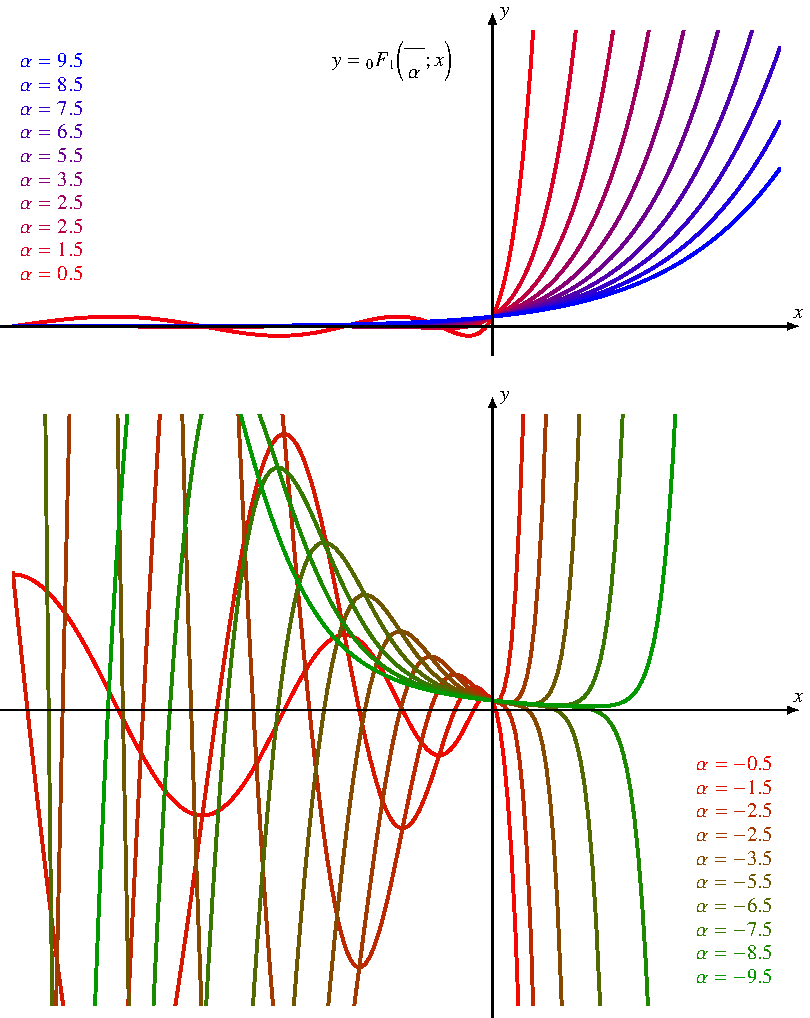
\includegraphics{chapters/040-rekursion/images/0f1.pdf}
\caption{Graphen der Funktionen $\mathstrut_0F_1(;\alpha;x)$ für
verschiedene Werte von $\alpha$.
\label{buch:rekursion:hypergeometrisch:0f1}}
\end{figure}
Die Funktionen $\mathstrut_0F_1$ sind in den Beispielen mit der
beschränkten trigonometrischen Funktion $\sin x$ und mit der
exponentiell unbeschränkten Funktion $\sinh x$ mit dem gleichen
Wert des Parameters und nur einem Wechsel des Vorzeichens des
Arguments verbunden worden.
Die Graphen der Funktionen $\mathstrut_0F_1$, die in 
Abbildung~\ref{buch:rekursion:hypergeometrisch:0f1} dargestellt sind,
machen dieses Verhalten plausibel.
Es wird sich später zeigen, dass $\mathstrut_0F_1$ auch mit den Bessel-
und den Airy-Funktionen verwandt sind.
Kapitel~\ref{chapter:0f1} zeigt Möglichkeiten der Berechnung der
Funktion $\mathstrut_0F_1$.

%
% Ableitung und Stammfunktion
%
\subsection{Ableitung und Stammfunktion hypergeometrischer Funktionen
\label{buch:rekursion:hypergeometrisch:stammableitung}}
Sowohl Ableitung wie auch Stammfunktion einer hypergeometrischen
Funktion lässt sich immer durch hypergeometrische Reihen ausdrücken.
%
% Ableitung
%
\subsubsection{Ableitung}
\index{Ableitung!hypergeometrischer Funktionen}%
Wir gehen aus von der Funktion
\begin{equation}
f(x)
=
\mathstrut_nF_m\biggl(
\begin{matrix}a_1,\dots,a_n\\b_1,\dots,b_m\end{matrix};
x\biggr)
=
\sum_{k=0}^\infty
\frac{
(a_1)_k\cdot\ldots\cdot(a_n)_k
}{
(b_1)_k\cdot\ldots\cdot(b_m)_k
}
\frac{x^k}{k!}.
\label{buch:rekursion:hypergeometrisch:eqn:f}
\end{equation}
Die Ableitung von $f(x)$ ist
\[
f'(x)
=
\sum_{k=0}^\infty
\frac{
(a_1)_k\cdot\ldots\cdot(a_n)_k
}{
(b_1)_k\cdot\ldots\cdot(b_m)_k
}
\frac{x^{k-1}}{(k-1)!}
=
\sum_{k=1}^\infty
\frac{
(a_1)_{k+1}\cdot\ldots\cdot(a_n)_{k+1}
}{
(b_1)_{k+1}\cdot\ldots\cdot(b_m)_{k+1}
}
\frac{x^k}{k!}.
\]
Der Koeffizient besteht zwar aus lauter Pochhammer-Symbolen, aber sie
haben jeweils zu einen Faktor zuviel.
Indem man den jeweils ersten Faktor ausklammert, kann man die
Terme wieder in die Form einer hypergeometrischen Reihe bringen.
\begin{align*}
f'(x)
&=
\sum_{k=1}^\infty
\frac{
a_1(a_1)_{k}\cdot\ldots\cdot a_n(a_n)_{k}
}{
b_1(b_1)_{k}\cdot\ldots\cdot b_m(b_m)_{k}
}
\frac{x^k}{k!}
\\
&=
\sum_{k=1}^\infty
\frac{
a_1\cdot\ldots\cdot a_n
}{
b_1\cdot\ldots\cdot b_m
}
\frac{
(a_1+1)_{k}\cdot\ldots\cdot(a_n+1)_{k}
}{
(b_1+1)_{k}\cdot\ldots\cdot(b_m+1)_{k}
}
\frac{x^k}{k!}
\\
&=
\frac{
a_1\cdot\ldots\cdot a_n
}{
b_1\cdot\ldots\cdot b_m
}
\,
\mathstrut_nF_m\biggl(
\begin{matrix}a_1+1,\dots,a_n+1\\b_1+1,\dots,b_m+1\end{matrix};
x\biggr).
\end{align*}

\begin{beispiel}
\index{Kosinus-Funktion}%
Die Kosinus-Funktion
\[
\cos x
=
1 - \frac{x^2}{2!} + \frac{x^4}{4!} - \frac{x^6}{6!} + \dots
=
\sum_{k=0}^\infty
\frac{(-1)^k}{(2k)!}x^{2k}
\]
kann wie folgt als hypergeometrische Funktion geschrieben werden.
Der Nenner hat $2k$ Faktoren, er muss also aus zwei Pochhammer-Symbolen
zusammengesetzt werden.
Dazu muss er erst um den Faktor $2^{2k}$ gekürzt werden, was
\[
\frac{(2k)!}{2^{2k}}
=
\frac12\cdot\frac32\cdot\frac52\cdot\ldots\cdot\frac{2k-1}2
\cdot
\frac22\cdot\frac42\cdot\frac62\cdot\ldots\cdot\frac{2k}2
=
({\textstyle\frac12})_k\cdot k!.
\]
Damit kann jetzt die Kosinus-Funktion als
\begin{align*}
\cos x
&=
\sum_{k=0}^\infty
\frac{2^k}{(2k)!}\biggl(\frac{-x^2}{4}\biggr)^k
=
\sum_{k=0}^\infty
\frac{1}{(\frac12)_k}
\frac{1}{k!}\biggl(\frac{-x^2}{4}\biggr)^k
=
\mathstrut_0F_1\biggl(\begin{matrix}\text{---}\\\frac12\end{matrix};-\frac{x^2}4\biggr)
\end{align*}
geschrieben werden kann.

Die Ableitung der Kosinus-Funktion ist daher
\begin{align*}
\frac{d}{dx} \cos x
&=
\frac{d}{dx}
\mathstrut_0F_1\biggl(
\begin{matrix}\text{---}\\\frac12\end{matrix};-\frac{x^2}4
\biggr)
=
\frac{1}{\frac12}
\,
\mathstrut_0F_1\biggl(
\begin{matrix}\text{---}\\\frac32\end{matrix};-\frac{x^2}4
\biggr)
\cdot\biggl(-\frac{x}2\biggr)
=
-x
\cdot
\mathstrut_0F_1\biggl(
\begin{matrix}\text{---}\\\frac32\end{matrix};-\frac{x^2}4
\biggr).
\intertext{Dies stimmt mit der in
\eqref{buch:rekursion:hypergeometrisch:eqn:sinhyper}
gefundenen Darstellung der Sinusfunktion mit Hilfe der hypergeometrischen
Funktion $\mathstrut_0F_1$ überein, es ist also wie erwartet}
&=-\sin x.
\qedhere
\end{align*}
\end{beispiel}

%
% Stammfunktion
%
\subsubsection{Stammfunktion}
\index{Stammfunktion!hypergeometrischer Funktionen}%
Eine Stammfunktion kann man auf die gleiche Art und Weise wie
die Ableitung finden.
Termweises Integrieren der Funktion
\eqref{buch:rekursion:hypergeometrisch:eqn:f}
ergibt
\begin{align}
\int f(x)\,dx
&=
\sum_{k=0}^\infty
\frac{
(a_1)_k\cdot\ldots\cdot(a_n)_k
}{
(b_1)_k\cdot\ldots\cdot(b_m)_k
}
\frac{x^{k+1}}{(k+1)!}.
\notag
\intertext{Wieder muss man die Pochhammer-Symbole durch solche mit
einem zusätzlichen Faktor schreiben.
Dies ist möglich, wenn keiner der Parameter $a_i=1$ und $b_j=1$
ist.
Die Stammfunktion wird daher
}
&=
\sum_{k=1}^\infty
\frac{
(a_1-1)(a_1)_k
\cdot\ldots\cdot
(a_n-1)(a_n)_k
}{
(b_1-1)(b_1)_k
\cdot\ldots\cdot
(b_m-1)(b_m)_k
}
\frac{x^k}{k!}
\notag
\\
&=
\sum_{k=1}^\infty
\frac{
(a_1-1)_{k+1}
\cdot\ldots\cdot
(a_n-1)_{k+1}
}{
(b_1-1)_{k+1}
\cdot\ldots\cdot
(b_m-1)_{k+1}
}
\frac{x^k}{k!}
\label{buch:rekursion:hypergeometrisch:eqn:stammfunktion:summe}
\\
&=
\mathstrut_nF_m\biggl(
\begin{matrix}
a_1-1,\dots,a_n-1\\
b_1-1,\dots,b_m-1
\end{matrix}
;x
\biggr)
-
\frac{(a_1-1)\dots(a_n-1)}{(b_1-1)\dots(b_m-1)}.
\notag
\end{align}
Der Term auf der rechten Seite kompensiert den konstanten
Term, der in der hypergeometrischen Funktion $\mathstrut_nF_m$
vorkommt, aber nicht in der
Summe~\eqref{buch:rekursion:hypergeometrisch:eqn:stammfunktion:summe}.

%
% Berechnung hypergeometrischer Funktionen
%
\subsection{Numerische Berechnung}
\begin{figure}
\centering
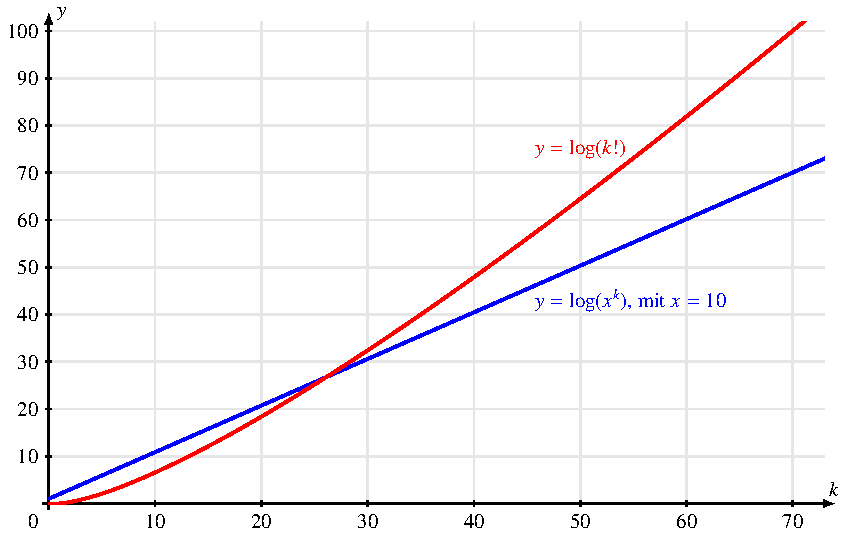
\includegraphics{chapters/040-rekursion/images/powergamma.pdf}
\caption{Anwachsen von Zähler $x^k$ und Nenner $k!$ in der
Exponentialreihe für $x=10$. 
Ab $k\approx 30$ werden die Terme der Reihe zunehmend kleiner,
was schliesslich zu Konvergenz der Reihe führt.
Für $k\approx 50$ sind die einzelnen Terme kleiner als die
Maschinengenauigkeit darzustellen gestattet.
Für negative $x$ wird starke Auslöschung die Genauigkeit des Resultates
unbrauchbar machen.
\label{buch:rekursion:hypergeometrisch:fig:powergamma}}
\end{figure}
Die naheliegendste Methode zur Berechnung einer hypergeometrischen
Funktion  $\mathstrut_pF_q$ ist die Auswertung der Potenzreihe.
Schon die einfachste hypergeometrische Funktion $\mathstrut_0F_0(x)=e^x$
zeigt aber, dass dabei numerische Schwierigkeiten auftreten können.
Für negative Argumente wird die Summe der Potenzreihe sehr klein.
Dies ist möglich, weil der Nenner $k!$ in der Potenzreihe
\[
\mathstrut_0F_0(x)
=
e^x
= 
1+x+\frac{x^2}{2!} + \frac{x^3}{3!} + \dots + \frac{x^k}{k!}+\dots
\]
sehr viel schneller anwächst als der Zähler $x^k$
(Abbildung~\ref{buch:rekursion:hypergeometrisch:fig:powergamma}).
Dazu muss aber $k$ eine gewisse Grösse haben, für $x=10$ muss
z.~B.~$k\gtrapprox30$ sein.
Für negative $x$ ist $e^x$ sehr klein, aber einzelne Terme in der
Summe sind viele Grössenordnungen grösser, was zu Auslöschung führt.

Im Falle der Exponentialfunktion gibt es eine einfache Lösung für
dieses Problem.
Um $y=e^x$ für negatives $x$ zu berechnen, verwendet man mit Vorteil
$y=1/e^{-x}$. Da $-x$ positiv ist, entsteht keine Auslöschung und der
Kehrwert führt ebenfalls keine weiteren Fehler ein.
So ist die Berechnung von $e^x$ auch für negative $x$ mit hoher
Genauigkeit möglich.

Ein ähnliches Phänomen muss ganz offensichtlich auch bei den
trigonometrischen Funktion $\sin x$ und $\cos x$ für beliebige
reelle Argumente auftreten.
Da diese Funktionen beschränkt sind, muss für grosse Absolutwerte
des Argumentes Auslöschung auftreten.
\index{Auslöschung}%
In diesem Fall können die Periodizität und goniometrische
\index{Periodizität}%
Identitäten verwendet werden, um die Berechnungsaufgabe in eine zu
transformieren, die mit hoher Genauigkeit ausgeführt werden kann.

Die allgemeine Theorie der hypergeometrischen Funktionen stellt
eine Reihe ähnlicher Transformationen bereit, die bei der Berechnung
ebenfalls hilfreich sein können.
Die Darstellung dieser Transformationen würde den Rahmen dieses
Buches sprengen.
Eine speziell interessante Technik, der Gausssche Kettenbruch,
\index{Gaussscher Kettenbruch}%
\index{Kettenbruch!Gaussscher}%
erlaubt Darstellungen einer Funktion als Kettenbruch zu finden, die
oft sehr gute numerische Eigenschaften haben.
Kapitel~\ref{chapter:0f1} untersucht einige dieser Möglichkeiten.


%\subsection{TODO}
%\begin{itemize}
%\item Hypergeometrische Transformationen
%\item Gausscher Kettenbruch \url{https://en.wikipedia.org/wiki/Gauss\%27s_continued_fraction}
%\end{itemize}
